\chapter{Planarity and Euler's formula}
\section*{Can the connections avoid crossings?}
A graph is planar if it can be drawn in the plane with edges meeting only at common endpoints. A crossing in one drawing does not prove non-planarity: the graph may have another crossing-free drawing. A planar drawing divides the plane into regions called faces, including the unbounded outside face.

\begin{figure}[htbp]
\centering
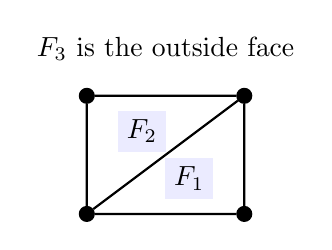
\begin{tikzpicture}[thick,vertex/.style={circle,draw=black,fill=black,inner sep=0pt,minimum size=5pt}]
\node[vertex] (a) at (0,0) {}; \node[vertex] (b) at (2,0) {}; \node[vertex] (c) at (2,1.5) {}; \node[vertex] (d) at (0,1.5) {};
\draw (a)--(b)--(c)--(d)--(a) (a)--(c);
\node[draw=none,rectangle,fill=blue!8] at (1.3,0.45) {$F_1$};
\node[draw=none,rectangle,fill=blue!8] at (0.7,1.05) {$F_2$};
\node[draw=none,rectangle,fill=white] at (1,2.1) {$F_3$ is the outside face};
\end{tikzpicture}
\caption{A crossing-free drawing has three faces: two inside and one outside.}
\end{figure}

\begin{theorem}[\Core{} Euler's formula]
For a connected planar graph with $v$ vertices, $e$ edges and $f$ faces, $v-e+f=2$.
\end{theorem}
\begin{figure}[htbp]
\centering
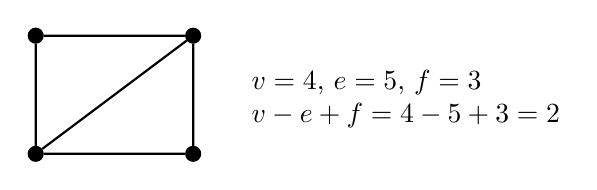
\begin{tikzpicture}[thick,vertex/.style={circle,draw=black,fill=black,inner sep=0pt,minimum size=5pt}]
\node[vertex] (a) at (0,0) {}; \node[vertex] (b) at (2,0) {}; \node[vertex] (c) at (2,1.5) {}; \node[vertex] (d) at (0,1.5) {};
\draw (a)--(b)--(c)--(d)--(a) (a)--(c);
\node[draw=none,rectangle,fill=white,align=left] at (4.7,0.7) {$v=4$, $e=5$, $f=3$\\$v-e+f=4-5+3=2$};
\end{tikzpicture}
\caption{Euler's formula counts vertices, edges, and faces in a planar embedding.}
\end{figure}
\begin{proof}
If the graph is a tree, it has $e=v-1$ and exactly one face, so $v-e+f=v-(v-1)+1=2$. Otherwise it contains a cycle. Delete an edge on a cycle. The graph stays connected, and the two faces on either side of that edge merge; thus $v$ decreases by 0, $e$ by 1 and $f$ by 1, leaving $v-e+f$ unchanged. Continue deleting cycle edges until a spanning tree remains. The tree case gives 2, so the original also gives 2.
\end{proof}

\Challenge{} If a plane graph has $c$ connected components, then
\[
v-e+f=1+c.
\]
To see this, first take a spanning forest: it has $v-c$ edges and one face. Adding each remaining edge within a component creates one cycle and splits one face into two, increasing both $e$ and $f$ by 1. Thus $v-e+f=v-(v-c)+1=1+c$.

For a simple connected planar graph with $v\geq 3$, each face boundary has at least three edge-sides, and each edge contributes two sides in total. Thus $3f\leq 2e$. Combining with Euler's formula gives $e\leq 3v-6$. If the graph is bipartite, every face boundary has at least four edge-sides, so $4f\leq 2e$ and $e\leq 2v-4$.

\Challenge{} The graph $K_5$ has $v=5,e=10$, exceeding $3v-6=9$, so it is not planar. The graph $K_{3,3}$ has $v=6,e=9$, exceeding the bipartite planar bound $2v-4=8$, so it too is non-planar.

\section*{\Challenge{} Stronger tests from faces}
The face-counting argument extends beyond triangular faces. The \emph{girth} of a graph is the length of its shortest cycle. If a connected simple planar graph has a cycle and girth $g\geq 3$, every face boundary has at least $g$ edge-sides. Since all $2e$ edge-sides are counted around faces, $gf\leq 2e$. Combining this with Euler's formula gives
\[
e\leq \frac{g}{g-2}(v-2).
\]
For $g=3$ this is the usual bound $e\leq 3v-6$; for a bipartite graph, $g\geq 4$ and it gives $e\leq 2v-4$. If the graph is a tree, the same bounds needed here follow directly from $e=v-1$.

This also gives an olympiad-style degree argument. A simple planar graph with $v\geq 3$ has a vertex of degree at most 5: otherwise every degree is at least 6, so the handshaking lemma gives $2e\geq 6v$, contradicting $e\leq 3v-6$. The argument applies to every subgraph as well, since subgraphs of planar graphs are planar.

\section*{\Uni{} Euler characteristic beyond the plane}
The planar formula is the genus-zero case of a broader topological statement. If a connected graph is embedded on an orientable surface of genus $h$ so that every face is a disk (a \emph{cellular embedding}), then
\[
v-e+f=2-2h.
\]
The sphere has genus $0$, giving Euler's formula; a torus has genus $1$, giving $v-e+f=0$. The term $2-2h$ is the Euler characteristic of the surface. This viewpoint is useful in university graph theory and topology; no surface theory is assumed elsewhere in this booklet.

For a connected simple graph with $v\geq 3$ cellularly embedded on this surface, counting at least three edge-sides around each face gives the corresponding bound $e\leq 3v-6+6h$ (with the tree case immediate). At genus zero this is the planar bound; increasing the genus allows more edges without crossings on the surface.

\textbf{Famous result (statement only).} Kuratowski's theorem says a finite graph is planar exactly when it contains no subdivision of $K_5$ or $K_{3,3}$. A subdivision replaces edges by internally vertex-disjoint paths; the theorem is not proved here.

\section*{Exercises}
\begin{enumerate}
\item A connected planar graph has 8 vertices and 12 edges. Find its number of faces.
\item Use the simple planar bound to show that $K_6$ is non-planar.
\item Why does a tree have one face when drawn in the plane without crossings?
\item \Challenge{} Show that every simple planar graph has a vertex of degree at most 5.
\end{enumerate}
